%!TEX root = ../thesis.tex
%*******************************************************************************
%*********************************** Analysis Overview *********
%*******************************************************************************

\titleformat{\chapter}[display]
	{\normalfont\LARGE}
	{\filleft\MakeUppercase{\chaptertitlename}\hspace{0.5cm}\rlap{\resizebox{!}{1.5cm}{\thechapter}~\rule{5cm}{1.5cm}}\hspace{2.0cm}}
  	{10pt}
  	{\bf\LARGE\filright}
\titlespacing*{\chapter}{0pt}{30pt}{20pt}


\chapter{Simplified likelihoods}\label{ch:simplify}

\ifpdf
    \graphicspath{{chapter-simplify/Figs/Raster/}{chapter-simplify/Figs/PDF/}{chapter-simplify/Figs/}}
\else
    \graphicspath{{chapter-simplify/Figs/Vector/}{chapter-simplify/Figs/}}
\fi

In the previous chapter, the concept of preserving an analysis for the purpose of reinterpretations has been introduced, and an example of a fully preserved analysis pipeline using containerised workflows has been discussed. In large-scale reinterpretations involving a large number of \gls{susy} models to be tested against, the wall time needed for statistical inference can be a computational bottleneck and thus calls for simplifications of the statistical model of an analysis. This chapter therefore introduces the concept of \textit{simplified likelihoods} as approach to approximate the statistical model of an analysis.

\section{Motivation}\label{sec:simplified_likelihood_motivation}

Reinterpretations of ATLAS SUSY searches in more complete and realistic \gls{susy} scenarios (as opposed to simplified models) often involves high-dimensional parameter spaces that are computationally extremely challenging to sample and compare to ATLAS data in an exhaustive way. Large-scale reinterpretations of this type have already been performed in ATLAS after the Run~1 data-taking period in both the 19-dimensional \gls{pmssm}~\cite{SUSY-2014-08} (introduced in~\cref{sec:theory_pmssm}) as well as a 5-dimensional representation of the \gls{pmssm}~\cite{Aaboud:2016wna}. Due to the complexity of the statistical models of today's SUSY searches in ATLAS, originating from the large number of channels and the large amount of nuisance parameters typically considered, the wall time needed for the statistical inference is usually far from negligible. In a typical large-scale reinterpretation involving $\mathcal{O}(10^5-10^6)$ sampled models, an optimistic estimation of the wall time needed for the statistical inference per model of $\mathcal{O}(\SI{10}{\second}-\SI{e2}{\second})$ is too computationally expensive, especially when more than just a few ATLAS \gls{susy} searches are included.

One approach of alleviating this computational problem is to approximate the \gls{susy} searches through their model-independent limits published in conjunction with the model-dependent exclusion limits. By construction, the model-independent limits are derived using only cut-and-count signal regions without multi-bin or shape-fit setups, thus making minimal model assumptions. While computationally very fast, this approach naturally underestimates the true exclusion power of the respective analysis due to the fact that model-dependent properties are not exploited (as they typically are in the exclusion signal regions). \Cref{fig:single_bin} compares the exclusion contours obtained with the full set of exclusion signal regions (shown in orange) to the exclusion contours obtained using the discovery signal regions (shown in green), defined in~\cref{tab:SignalRegionDef}. As the discovery signal regions are not mutually exclusive, they are not statistically combined and thus three separate observed and expected contours can be drawn. From \cref{fig:single_bin}, it is clear that even a best-expected combination of the three discovery signal regions does not reach the sensitivity achieved using the two-dimensional shape-fit setup resulting from statistical combination of the nine exclusion signal regions. Nonetheless, this approach has been opted for in the large-scale scan of the \gls{pmssm} using ATLAS data from Run~1~\cite{SUSY-2014-08}, yielding conservative exclusion power and thus room for improvement.

Therefore, the following sections introduce a method for approximating ATLAS SUSY searches without disregarding their elaborate use of multi-bin signal regions exploiting the varying shapes of signal and \gls{sm} background distributions. 

\begin{figure}
	\centering
	\begin{subfigure}[b]{0.5\textwidth}
		\centering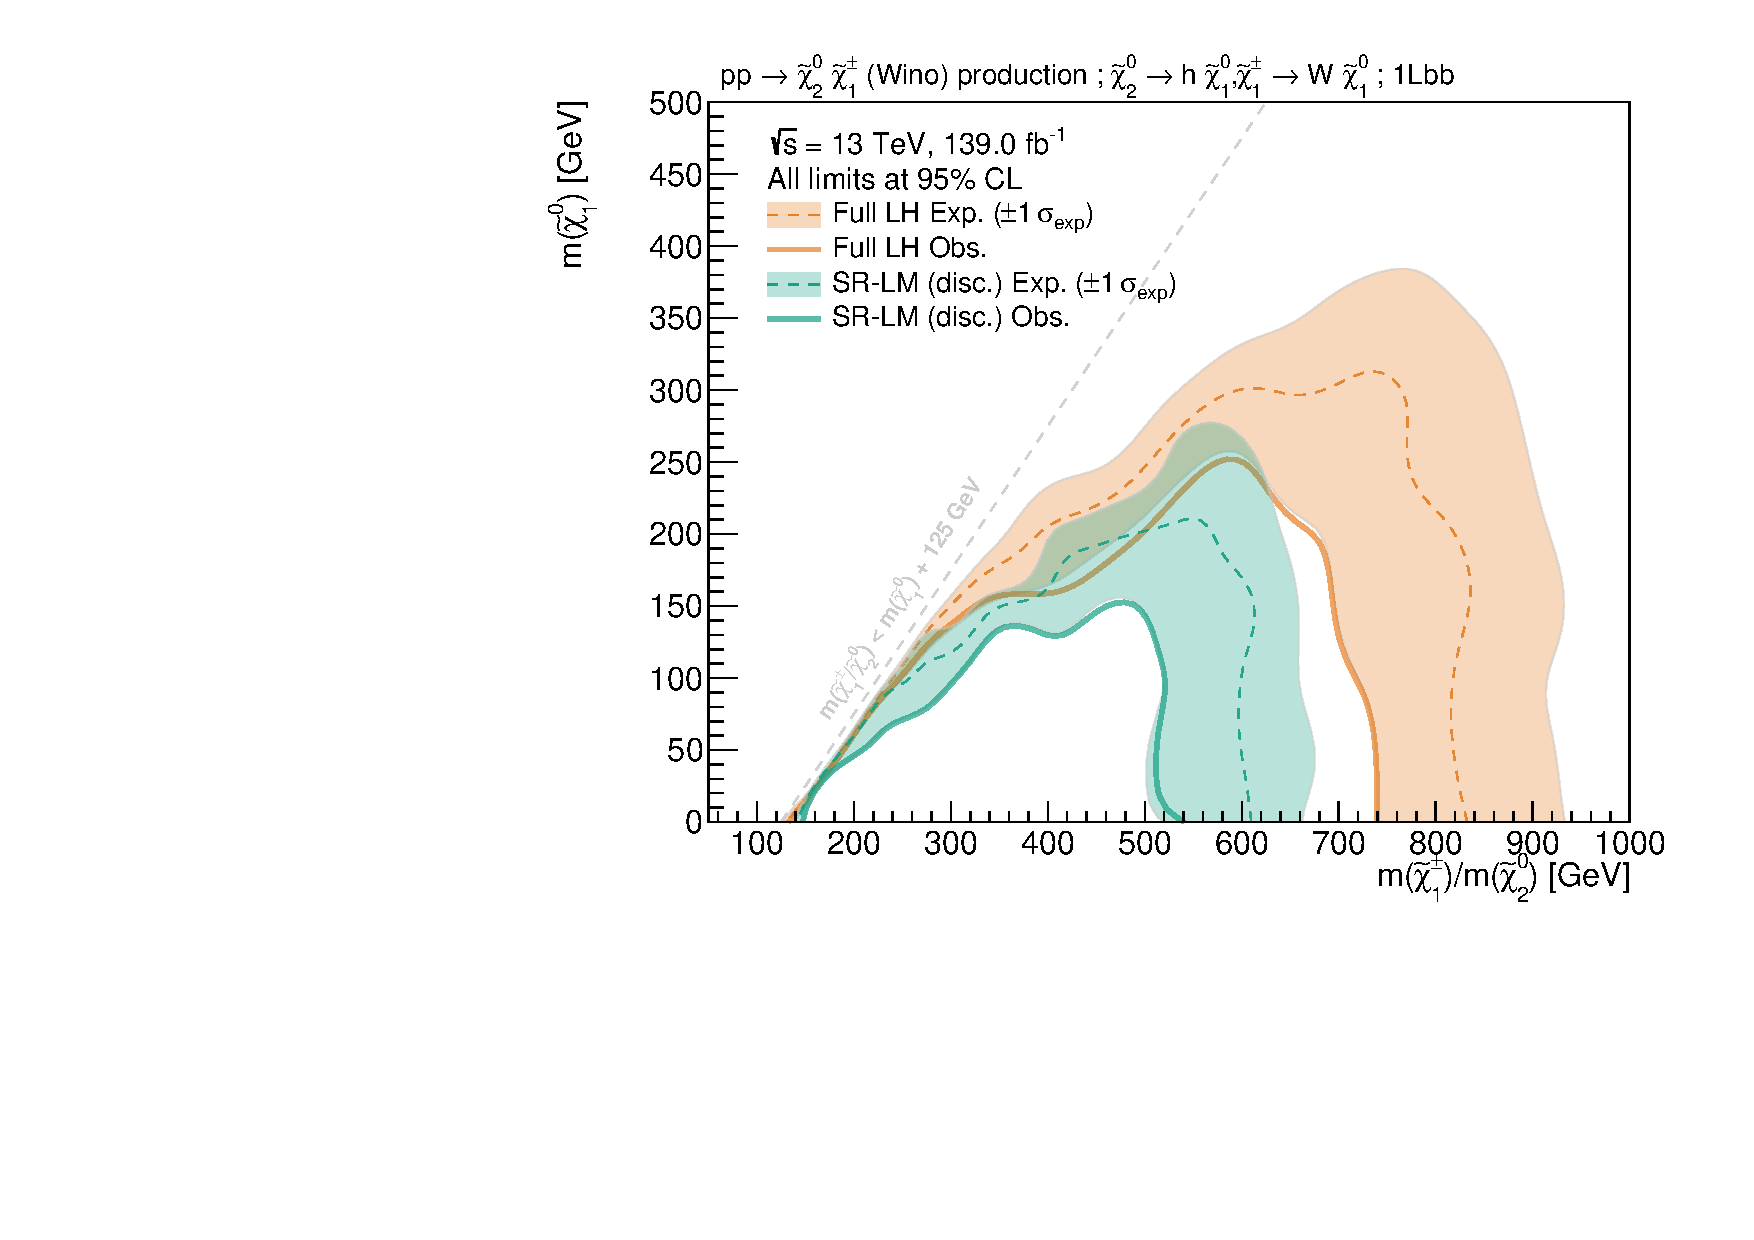
\includegraphics[width=\textwidth]{exclusion_1Lbb_SRLM_noLabel}
		\caption{Discovery SR-LM\label{fig:single_bin_SRLM}}
	\end{subfigure}\hfill
	\begin{subfigure}[b]{0.5\textwidth}
		\centering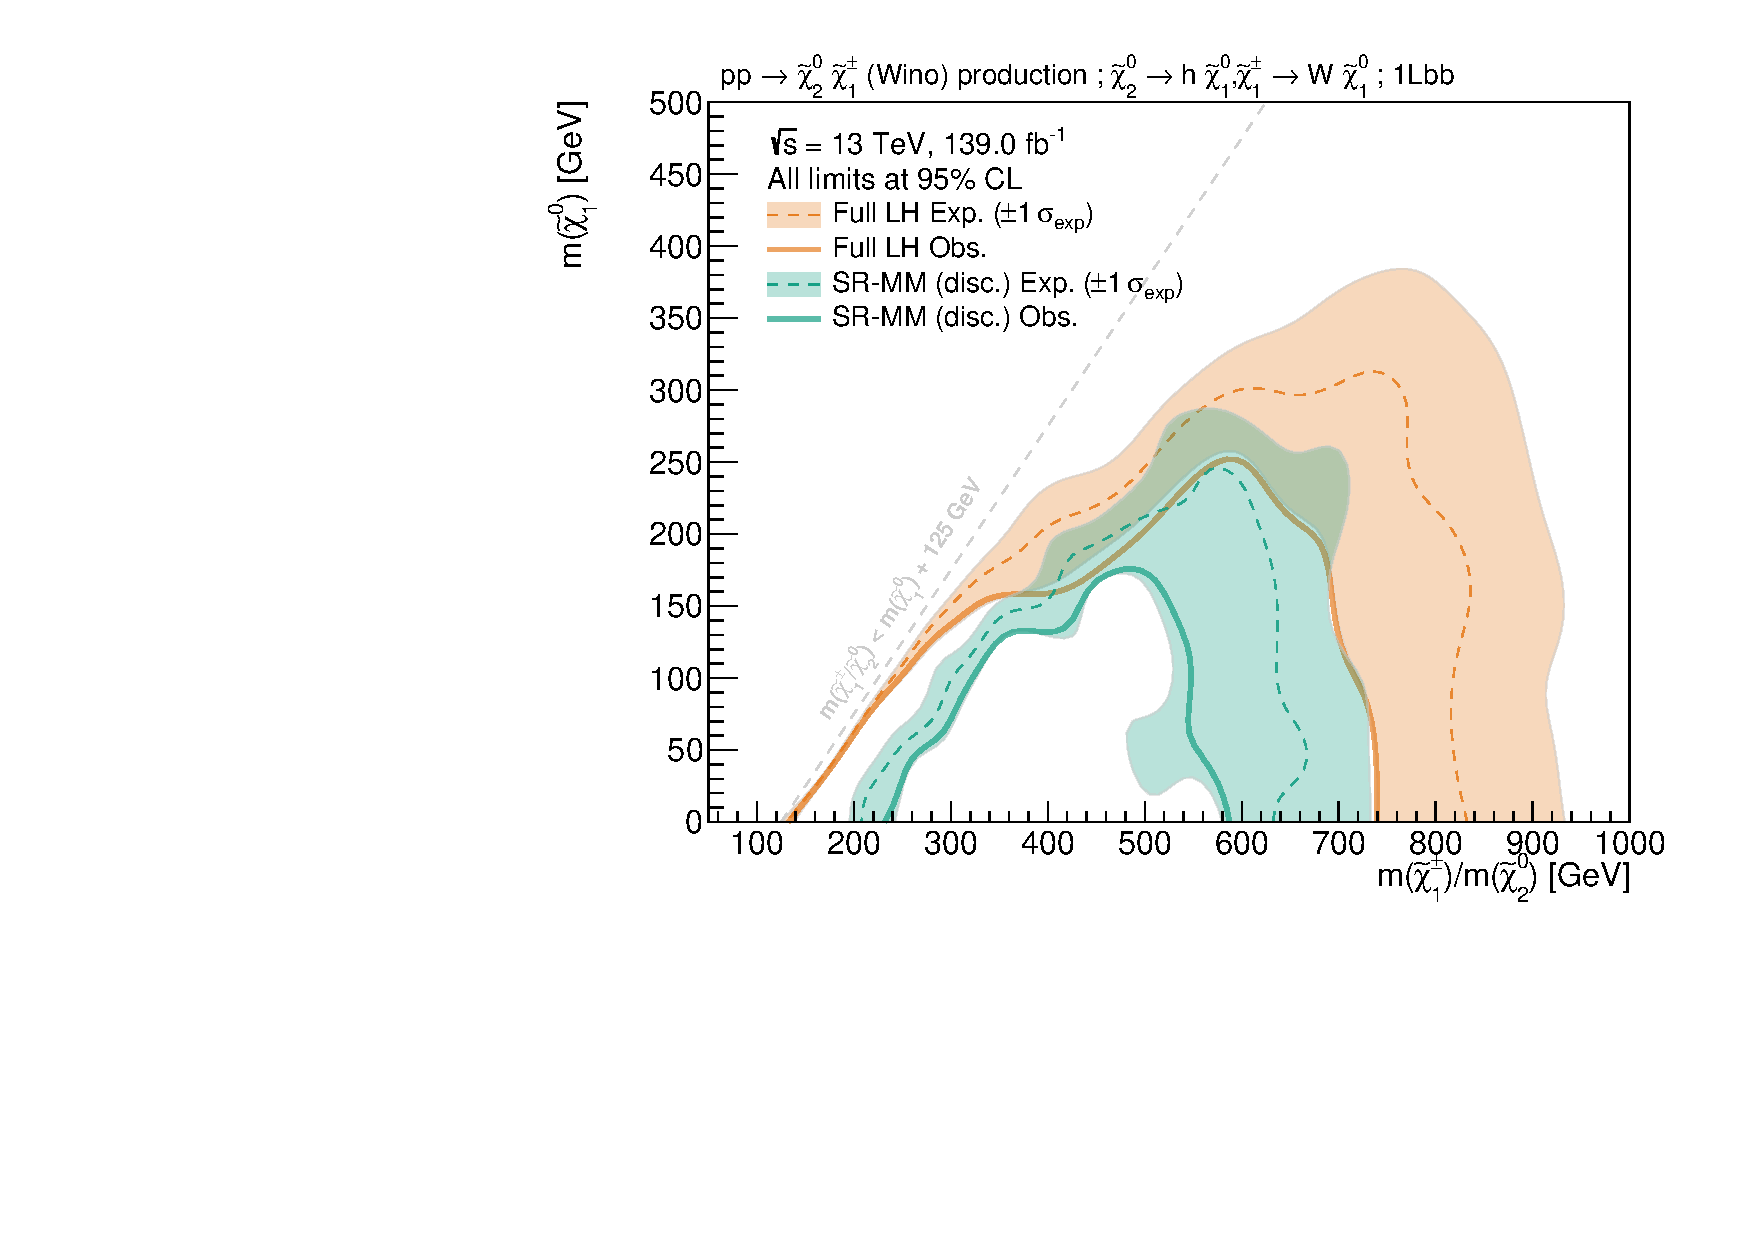
\includegraphics[width=\textwidth]{exclusion_1Lbb_SRMM_noLabel}
		\caption{Discovery SR-MM\label{fig:single_bin_SRMM}}
	\end{subfigure}\hfill
	\begin{subfigure}[b]{0.5\textwidth}
		\centering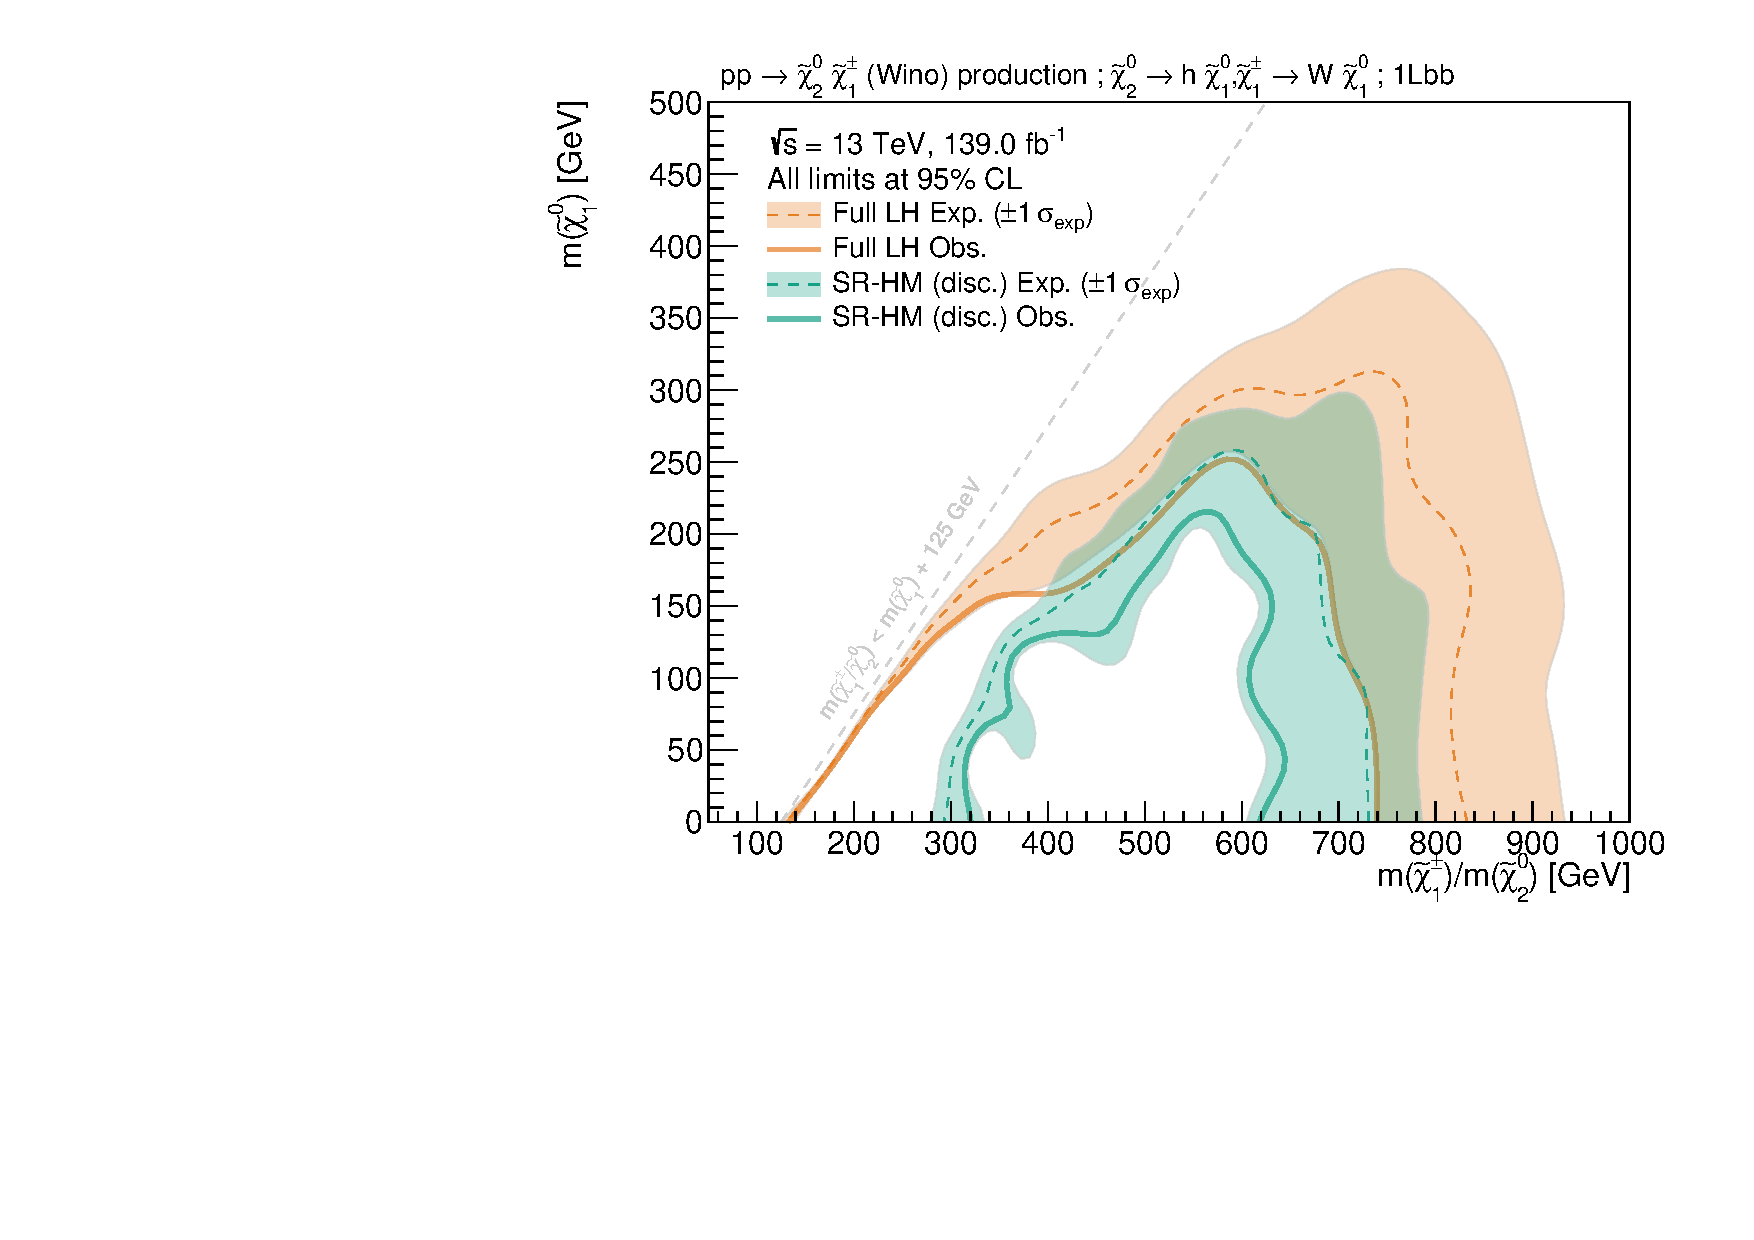
\includegraphics[width=\textwidth]{exclusion_1Lbb_SRHM_noLabel}
		\caption{Discovery SR-HM\label{fig:single_bin_SRHM}}
	\end{subfigure}%
	\caption{Comparison of exclusion limits obtained using a likelihood built from all nine exclusion signal regions (orange), and the discovery signal regions (green). As discussed in~\cref{sec:signal_region_definitions}, the discovery signal regions are simple cut-and-count regions with minimal model assumptions. They are not mutually exclusive, they cannot be fitted together, thus resulting in three separate exclusion contours. All statistical and systematic uncertainties on the background and the signal event rates are included.}\label{fig:single_bin}
\end{figure}

\section{Building simplified likelihoods}\label{sec:building_simplified_likelihoods}



In order to retain the full statistical combination of multiple signal region bins implemented in many SUSY searches, while still being able to achieve a sufficiently fast approximation, the statistical treatment of the systematic uncertainties as well as of the background model needs to be simplified. In the procedure presented in the following, this is achieved by first performing a background-only fit to data in all \glspl{sr} and \glspl{cr}, in order to determine the best-fit values of all the model parameters $\boldsymbol{\phi}$. This allows to calculate the post-fit total background estimate as well as the total uncertainty on the estimate in every bin, both of which can be used to construct a simplified likelihood.

As the full likelihood in \texttt{JSON} format defines the full statistical model used for the statistical inference, the above background-only fit can be performed using \texttt{pyhf} and the preserved full likelihood of the analysis. With the full likelihoods starting to become available on \textsc{HEPData} (see \eg \reference\cite{fullLH_1Lbb}) this procedure can rely on public information only and is therefore widely accessible to the \gls{hep} community. The simplified likelihoods introduced in the following, follow the same \texttt{JSON} specification introduced for the full likelihoods in \reference\cite{ATL-PHYS-PUB-2019-029}. The following description highlights the specification details relevant to the simplified likelihood. 

\subsubsection{Background model}

In the simplified likelihood, the background model is approximated with a single background sample, representing the total \gls{sm} background estimate in the different analysis channels (called \texttt{total\_bkg} in \cref{lst:bkg_sample}). The sample rate of the total background sample is set to the total post-fit background estimate obtained in the background-only fit using the full statistical model (in \cref{lst:bkg_sample} set to be $10.0$). Likewise, the complete set of nuisance parameters in the original full likelihood is reduced to a single constrained parameter $\alpha$ with up and down variations corresponding to the post-fit uncertainties on the total \gls{sm} background estimates in each bin (called \texttt{total\_error} in \cref{lst:bkg_sample}). It is constrained by a Gaussian $\mathrm{Gaus}(a = 0 \vert \alpha , \sigma = 1)$ and is correlated over all bins in each channel. Although the final uncertainty is constrained by a simple Gaussian, the full treatment of the uncertainties in the background-only fit using the full likelihood ensures that non-Gaussian effects are included to some extent.

\begin{minipage}{\linewidth}
\begin{lstlisting}[language=json,firstnumber=1,caption={Example of a total background sample with sample rate and total uncertainty as derived from a previous fit in the \glspl{sr} and \glspl{cr}.},captionpos=b, label=lst:bkg_sample]
{
	"name": "total_bkg",
	"data": [10.0],
	"modifiers": [{"data": {"hi_data": [12.0], "lo_data": [8.0]}, "name": "total_error", "type": "histosys"}]
}
\end{lstlisting}
\end{minipage}

\subsubsection{Analysis channels}

Each original channel in the full likelihood with the original number of bins is also entering the simplified likelihood, and each contains the total background sample as specified above. Apart from the total background sample, one additional sample is needed---the signal sample. An example of a signal sample is shown in \cref{lst:sig_sample}. It introduces the unconstrained signal strength parameter $\mu$ as second parameter of the statistical model. For simplicity, the example shown in \cref{lst:sig_sample} does not introduce any additional uncertainties on the signal rates, thereby assuming that them to be negligible. Depending on the \gls{bsm} scenario, signal uncertainties can be introduced through additional nuisance parameters (modifiers).

\begin{minipage}{\linewidth}
\begin{lstlisting}[language=json,firstnumber=1,caption={Example of a signal sample with sample rate and unconstrained normalisation parameter.},captionpos=b, label=lst:sig_sample]
{
	"name": "signal",
	"data": [7.0],
	"modifiers": [{"data": null, "name": "mu_Sig", "type": "normfactor"}]
}
\end{lstlisting}
\end{minipage}

\subsubsection{Observations and measurements}

According to the \texttt{JSON} specification defined in \reference\cite{ATL-PHYS-PUB-2019-029}, the data observed by the analysis in each channel (and each bin) is introduced by means of an \textit{observation}. In the case of the simplified likelihood, this is taken directly from the full likelihood and, by construction, does not need to be modified. An example of an observation including several channels and bins is shown in~\cref{lst:observation}.

\begin{minipage}{\linewidth}
\begin{lstlisting}[language=json,firstnumber=1,caption={Example of an observation in the simplified likelihood. It can be directly taken from the corresponding full likelihood. This example implements three channels, two with one bin, and one with three bins.},captionpos=b, label=lst:observation]
{
	"observations": {
		{"name": "channel_A" : "data": [25.0]},
		{"name": "channel_B" : "data": [20.0]},
		{"name": "channel_C" : "data": [11.0, 13.0]}
	}	
}
\end{lstlisting}
\end{minipage}

The only part of the \texttt{JSON} specification left to be defined is the \textit{measurement}, specifying the name of the parameter of interest as well as parameter set configurations not already covered in the channel definitions. For the simplified likelihood, it is straightforward to write down, as can be seen in~\cref{lst:measurement}.

\begin{minipage}{\linewidth}
\begin{lstlisting}[language=json,firstnumber=1,caption={Example of a measurement in the simplified likelihood. The signal strength is the parameter of interest, no additional parameters need further configuration.},captionpos=b, label=lst:measurement]
{
	"measurements": {
		"name": "myMeasurement",
		"config": { "poi": "mu_Sig", "parameters": []}
	}	
}
\end{lstlisting}
\end{minipage}

Put together, the above pieces result in a simplified likelihood for a given signal model, using a background model obtained from an initial background-only fit using the full likelihood considering the full treatment of systematic uncertainties. Replacing the signal sample by the means of \texttt{JSON} patches allows for systematic reinterpretations of any signal model for which the expected rates in the analysis regions are known.  


\section{Computational performance}\label{sec:cpu_performance}

One of the main figures of merit of an analysis approximation naturally is the reduction in wall time compared to the full analysis. \Cref{fig:benchmark_1Lbb} shows a benchmark for different likelihood configurations of the search for electroweakinos presented herein. The wall time of the full analysis likelihood is compared with that of the simplified likelihood constructed following the previously introduced prescription. In addition, the wall time of the single-bin likelihood using the discovery \glspl{sr} in a setup similar to that already used in the naive approximation in \cref{fig:single_bin}, is shown. For each likelihood, different computational backends are used for the tensor algebra operations in \texttt{pyhf}. All benchmarks have been performed on an Intel i7-4790 CPU with a nominal clock speed of $\SI{3.60}{\GHz}$, 4 cores and 8 threads. The CPU was not isolated but under minimal load. The original 125 signal points of the analysis where used in each configuration.

\begin{figure}
	\centering    
	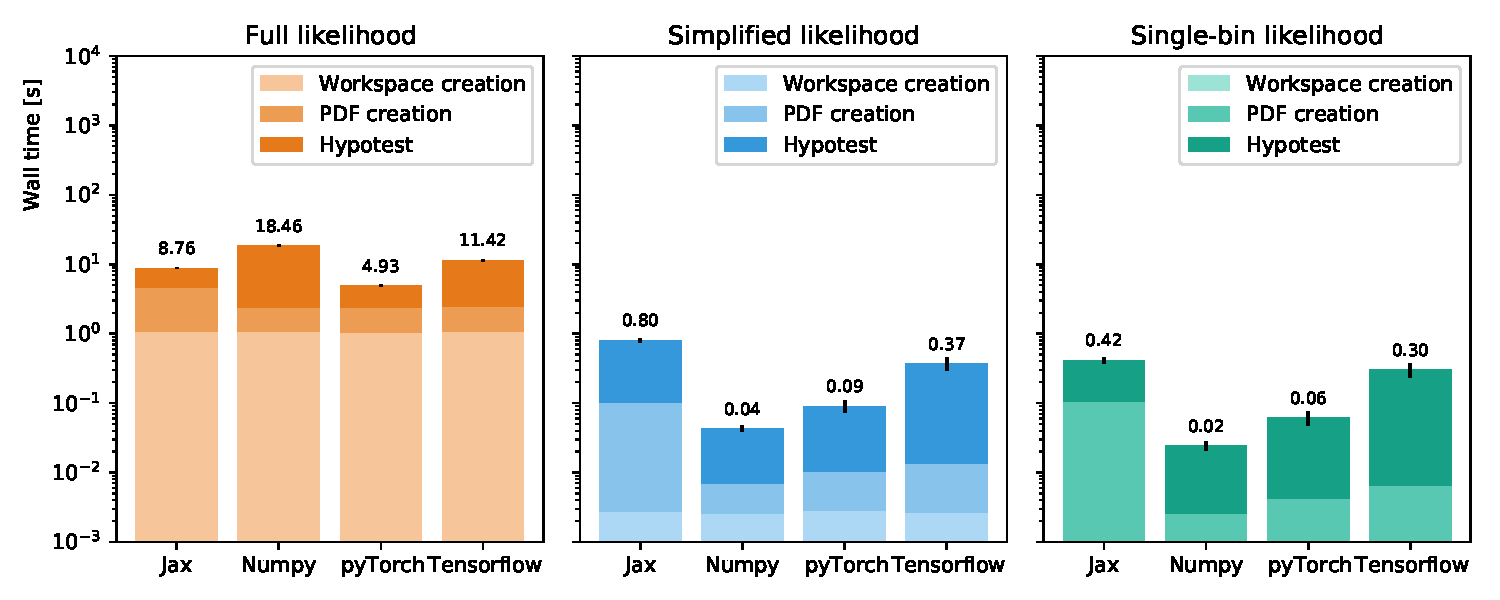
\includegraphics[width=\textwidth]{benchmark_1Lbb}
	\caption{Benchmarks of the CPU-time necessary for hypothesis testing using different likelihood and \texttt{pyhf} configurations in the context of the ATLAS 1L electroweakino search, run on a non-isolated CPU with 4 threads. The full likelihood (left) includes the full statistical implementation of the original analysis, the simplified likelihood (center) represents the simplified likelihood approach presented in this document, and the single-bin likelihood (right) represents a single-bin approximation of the ATLAS 1L electroweakino search. The uncertainties represent the standard deviation of the benchmark test sample.}\label{fig:benchmark}
	\label{fig:benchmark_1Lbb}
\end{figure}

The use of automatic differentiation of the full likelihood gradient enabled by some of the tensor algebra backends to \texttt{pyhf} offers an efficient minimisation of the likelihood resulting in fast hypothesis tests of $\mathcal{O}(\SI{5}{\second})$ for the full analysis. In large-scale reinterpretations, this is however still to computationally expensive. The simplified likelihood, on the other hand, results in a wall time for hypothesis tests as fast as $\SI{0.04}{\second}$ per signal model. Thus, the computational performance of the simplified likelihood is in the same order of magnitude as that of the naive single-bin approach\footnote{In fact, the simplified likelihood is actually even faster than the single-bin approach, as the latter needs to be executed separately for each discovery \gls{sr} and thus the numbers quoted need to be multiplied by the number of discovery \glspl{sr} used in the analysis.}, but offers by construction a significantly better approximation oft the true analysis exclusion power.

Interestingly, the wall time of the simplified likelihood does not benefit from the usage of features like automatic differentiation offered by \eg \textsc{PyTorch}. This is due to the extreme simplicity of the simplified likelihood function, therefore the computational benefits from features like automatic differentiation do not outweigh the overhead of libraries like \textsc{PyTorch}.

In addition to the search for electroweakinos presented herein, the simplified likelihood approach has also been applied on a number of other ATLAS SUSY searches. \Cref{tab:simplified_performance} summarises the mean wall time of all ATLAS \gls{susy} searches investigated using the simplified likelihood approach. In all cases, \textsc{PyTorch} offers the fastest backend for the full likelihood while \textsc{NumPy} performs best for the simplified likelihood. The performance improvement of roughly two orders of magnitude obtained in the 1-lepton analysis is confirmed in the other ATLAS \gls{susy} searches investigated. The wall time of the simplified likelihood appears to be bound from below at $\mathcal{O}(\SI{e-2}{\second})$, limiting the performance gain for some of the faster analyses.

\begin{table}
	\begin{center}
	\small
			\begin{tabular} {l r r r}
				\toprule
				Analysis & Full likelihood [s] & Simplified likelihood [s] & Improvement \\
				\midrule
				ATLAS compressed search~\cite{SUSY-2018-16} & $16.49\pm 3.16$ & $0.073 \pm 0.012$ & 236$\times$ \\
				ATLAS 3-lepton search & $40.41 \pm 15.7$ & $0.082 \pm 0.021$ & 495$\times$\\
				ATLAS 2-lepton search~\cite{SUSY-2018-32} & $5.93 \pm 0.16$ & $0.079 \pm 0.0082$ & 75$\times$\\
				ATLAS 1-lepton search~\cite{SUSY-2019-08} & $4.93 \pm 0.11$ & $0.040 \pm 0.0057$ & 123$\times$ \\
				ATLAS direct stau search~\cite{SUSY-2018-04} & $1.91 \pm 0.090$ & $0.039 \pm 0.0055$ & 49$\times$\\
				ATLAS sbottom search~\cite{SUSY-2018-31} & $1.36 \pm 0.067$ & $0.038 \pm 0.0046$ & 36$\times$ \\
				ATLAS stop search & $2.27 \pm 0.062$ & $0.044 \pm 0.011$ & 51$\times$\\
				\bottomrule
			\end{tabular}
		\caption{Benchmarks of the wall times (in seconds) needed for computing the CL$_s$ value for a single signal model using the full and the simplified likelihoods. The signal models used for the benchmarks include all signal models originally considered in the respective search. The uncertainty corresponds to the standard deviation of the benchmark sample. Additionally, the performance improvement is stated as ratio between the wall times. The benchmarks were performed on a non-isolated CPU under minimal load on a node without dedicated GPU. The \textsc{PyTorch} (\textsc{NumPy}) backend of \texttt{pyhf} is used for the full (simplified) likelihood, in conjunction with the \textsc{SciPy} optimiser. Searches without reference quoted are not yet public.}
		\label{tab:simplified_performance}
	\end{center}
\end{table}

\section{Physics performance}\label{sec:physics_performance}

A comparison of the exclusion contours obtained with the full and simplified likelihoods in the context of the search for electroweakinos presented herein is shown in~\cref{fig:results_simplify_1Lbb}. The results obtained using the simplified likelihood are shown in blue, while the results obtained using the full likelihood are presented in orange. Both the observed (without the usual theoretical up and down variations on the signal cross section) and expected exclusion limits including the uncertainty band are shown. In the case of the full likelihood, the complete set of \gls{mc} statistical and systematic uncertainties introduced in \cref{ch:uncertainties} are taken into account. As discussed in \cref{sec:building_simplified_likelihoods}, the uncertainty band on the simplified likelihood contour results from the single nuisance parameter built by reducing the original nuisance parameters.

\begin{figure}
\floatbox[{\capbeside\thisfloatsetup{capbesideposition={right,center},capbesidewidth=0.35\textwidth}}]{figure}[\FBwidth]
{\caption{Comparison of the simplified likelihood (blue contours) and full likelihood (orange contours) results for the search for electroweakinos presented previously. The observed contours are shown as solid lines, while the expected contours are shown as dashed lines. The uncertainty band includes all \gls{mc} statistical and systematic uncertainties in the case of the full likelihood, and only the simplified uncertainties in the case of the simplified likelihood.}\label{fig:results_simplify_1Lbb}}
{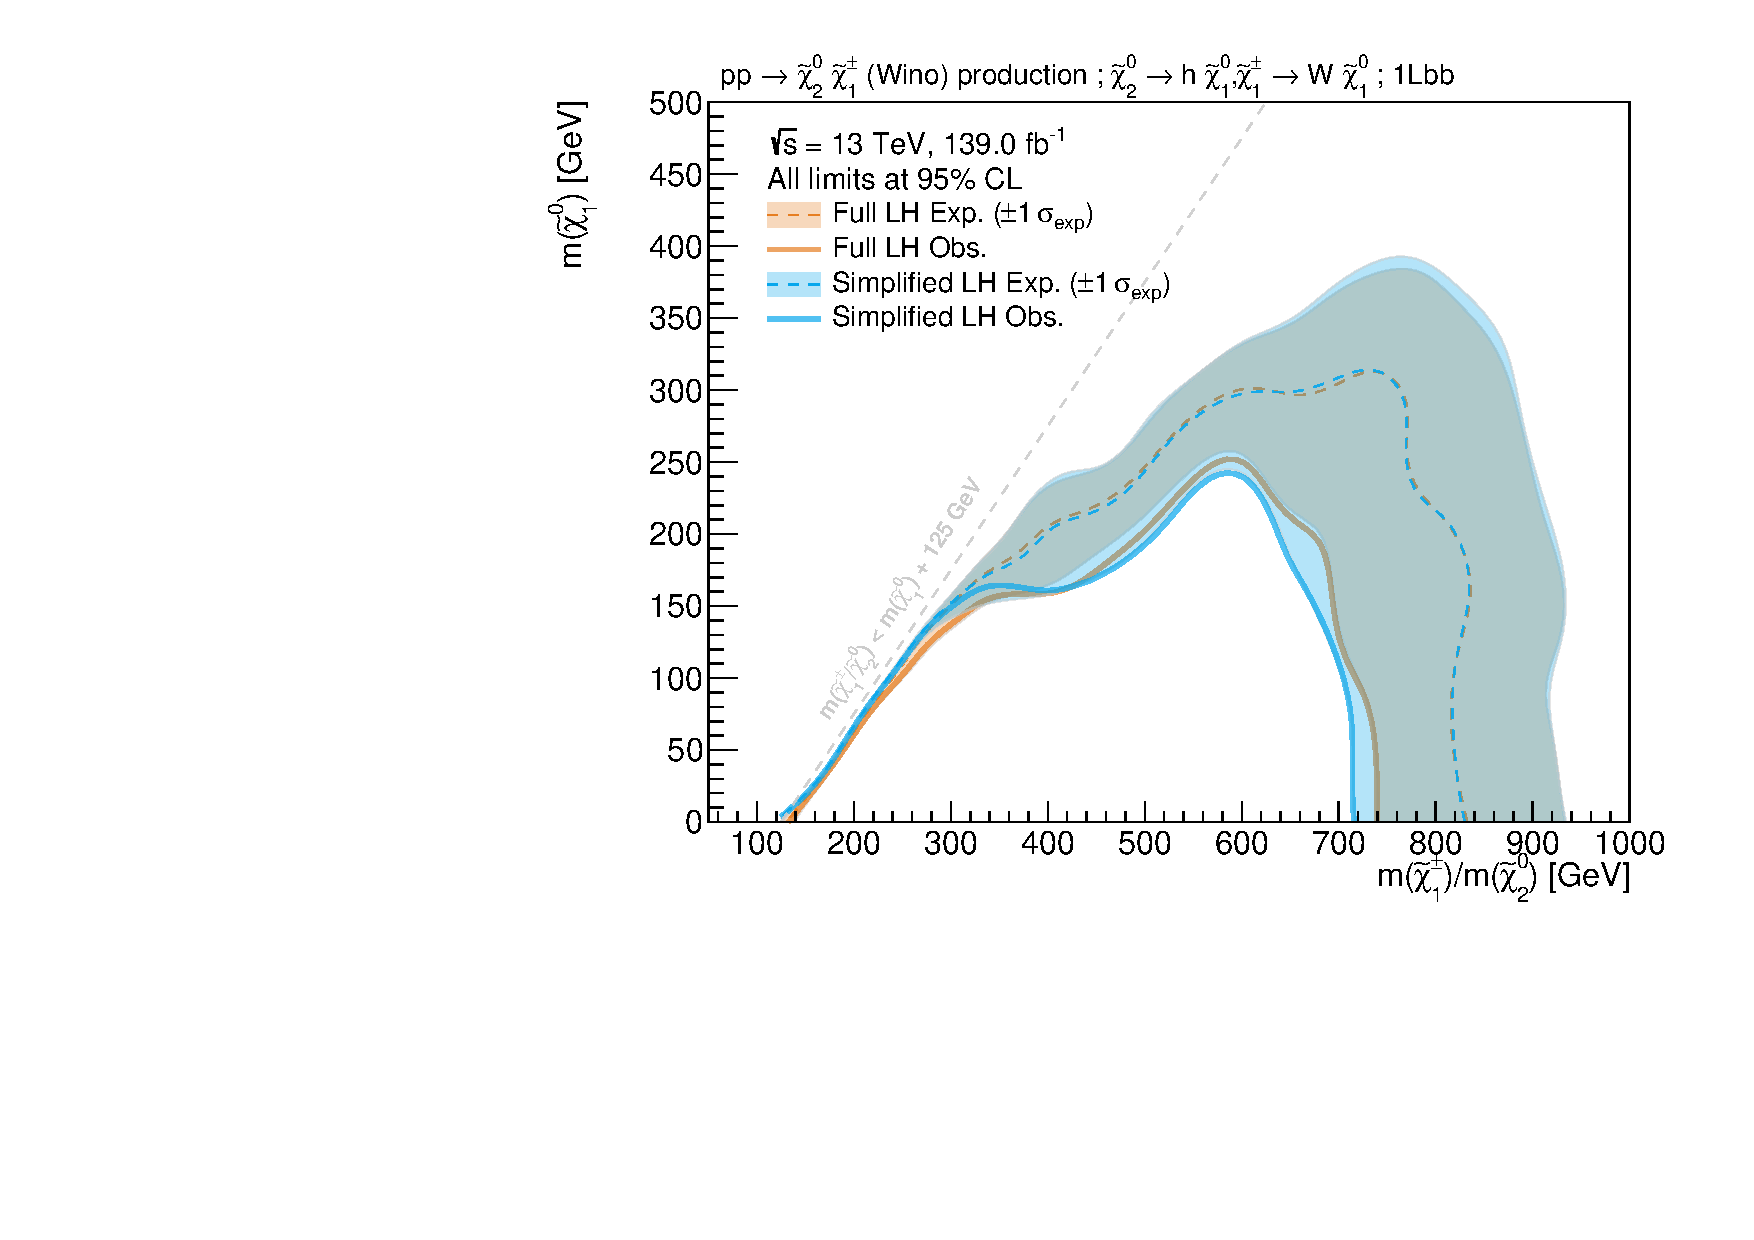
\includegraphics[width=0.60\textwidth]{exclusion_1Lbb_noLabel}}
\end{figure}

The exact observed and expected CL$_s$ values obtained using both likelihoods are shown in~\cref{fig:scatter_cls}. As expected from the exclusion contour, both the simplified and the full likelihood agree reasonably well across the majority of the shown range in CL$_s$. For signal models well within exclusion with the full likelihood, \ie $\mathrm{CL}_s \ll 0.05$, the simplified likelihood of the 1-lepton analysis tends to result in slightly lower CL$_s$ values than the full likelihood, thus giving a slightly too optimistic sensitivity estimate. In the range relevant to the exclusion contour at 95\% CL, the results from the simplified likelihood agree however well with those from the full likelihood.

In addition to the 1-lepton search, the simplified likelihood approach has been applied on the ATLAS \gls{susy} searches listed in \cref{tab:simplified_performance}. An overview of the results can be seen in~\cref{fig:results_analyses}, comparing the exclusion contours obtained with the simplified likelihood against the full analysis results. In some analyses, \eg the ATLAS sbottom search as well as the ATLAS 3-lepton search, the simplified likelihoods show excellent agreements. In other analyses like \eg the ATLAS direct stau search, the agreement is less good but overall still acceptable, demonstrating that this method can offer a fast and reliable approximation of ATLAS \gls{susy} searches.


\begin{figure}
	\centering
	\begin{subfigure}[b]{0.5\textwidth}
		\centering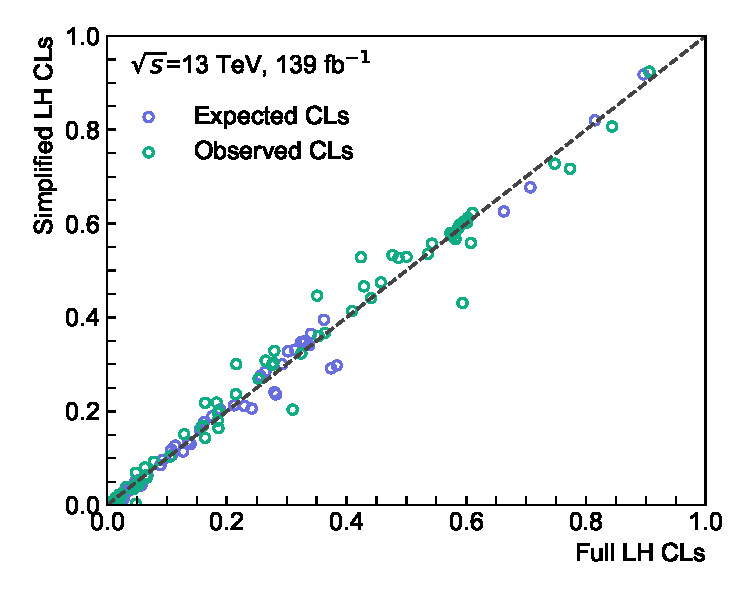
\includegraphics[width=\textwidth]{cls_scatter_1Lbb_lin}
		\caption{Linear scale}
	\end{subfigure}\hfill
	\begin{subfigure}[b]{0.5\textwidth}
		\centering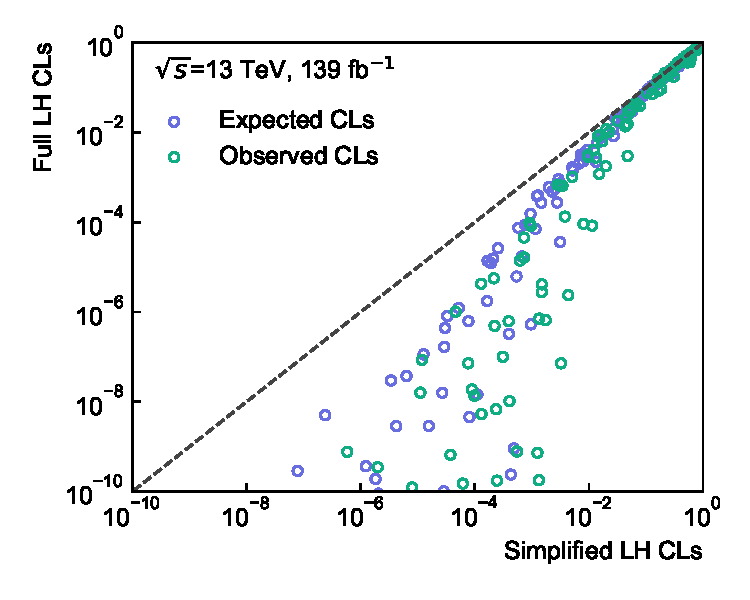
\includegraphics[width=\textwidth]{cls_scatter_1Lbb_log}
		\caption{Logarithmic scale}
	\end{subfigure}
	\caption{Scatter plots comparing the observed and expected CL$_s$ values obtained using the simplified and the full likelihoods for the same set of signal models considered in the search for electroweakinos. Both linear and logarithmic scale representations are shown.}\label{fig:scatter_cls}
\end{figure}


\begin{figure}
	\centering
	\begin{subfigure}[b]{0.5\textwidth}
		\centering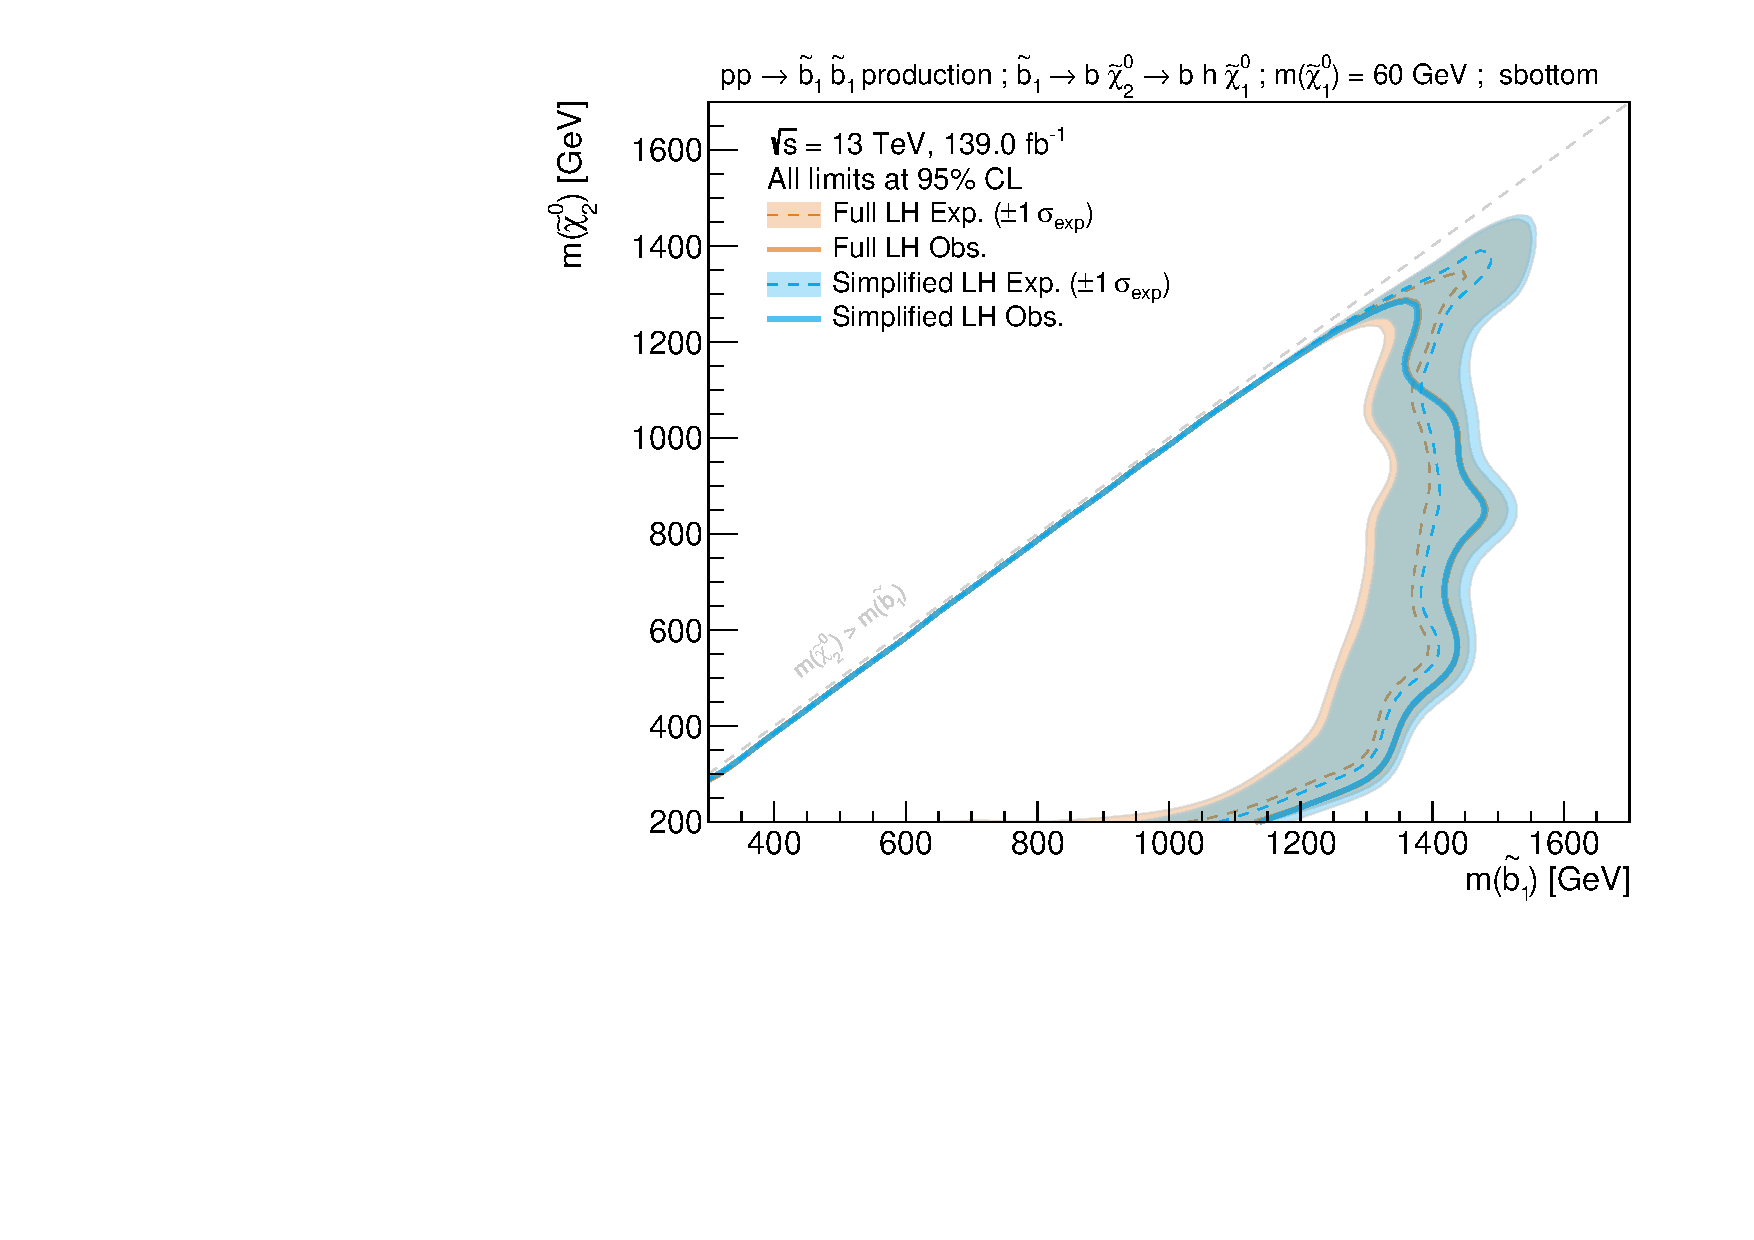
\includegraphics[width=\textwidth]{exclusion_sbottom_noLabel}
		\caption{ATLAS sbottom search~\cite{SUSY-2018-31}\label{fig:results_sbottom}}
	\end{subfigure}\hfill
	\begin{subfigure}[b]{0.5\textwidth}
		\centering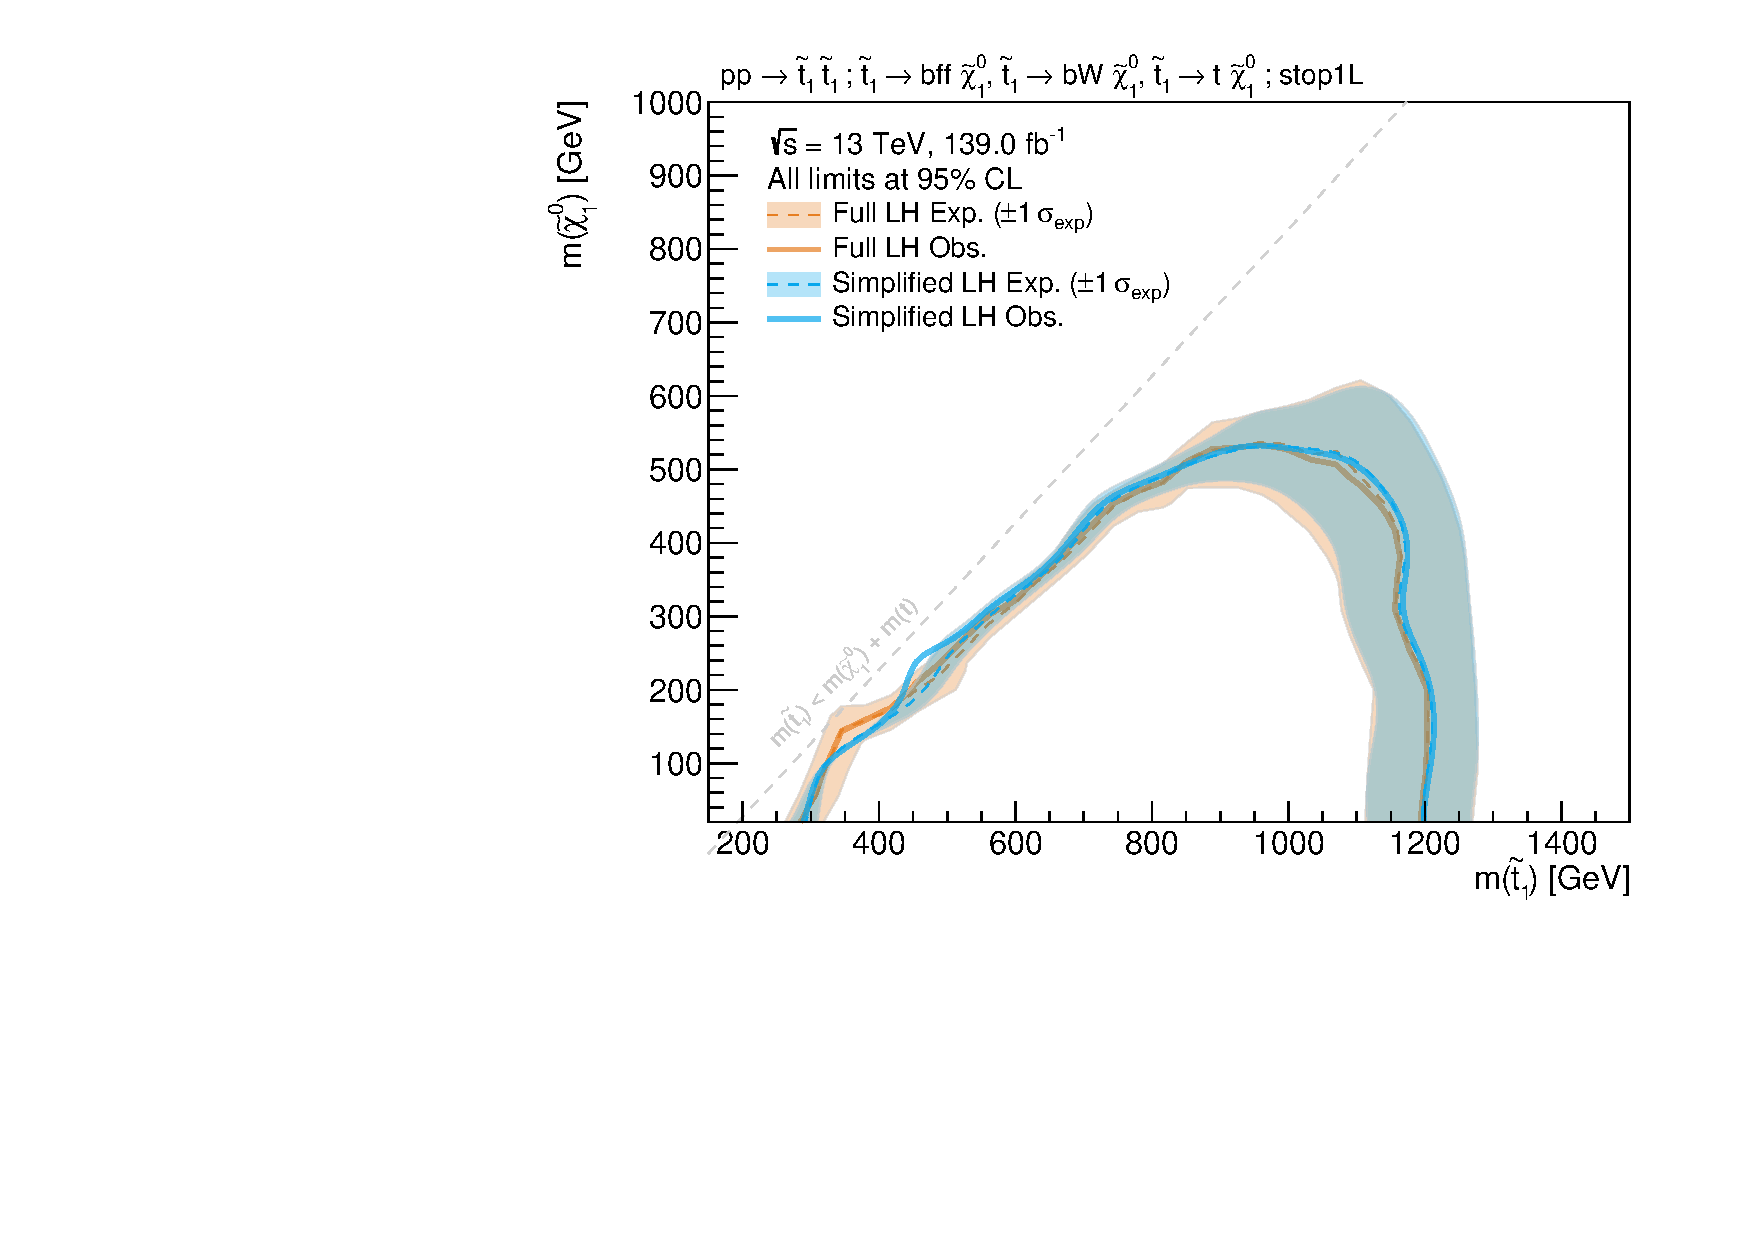
\includegraphics[width=\textwidth]{exclusion_stop1L_noLabel}
		\caption{ATLAS stop search\label{fig:results_stop1L}}
	\end{subfigure}\hfill
	\begin{subfigure}[b]{0.5\textwidth}
		\centering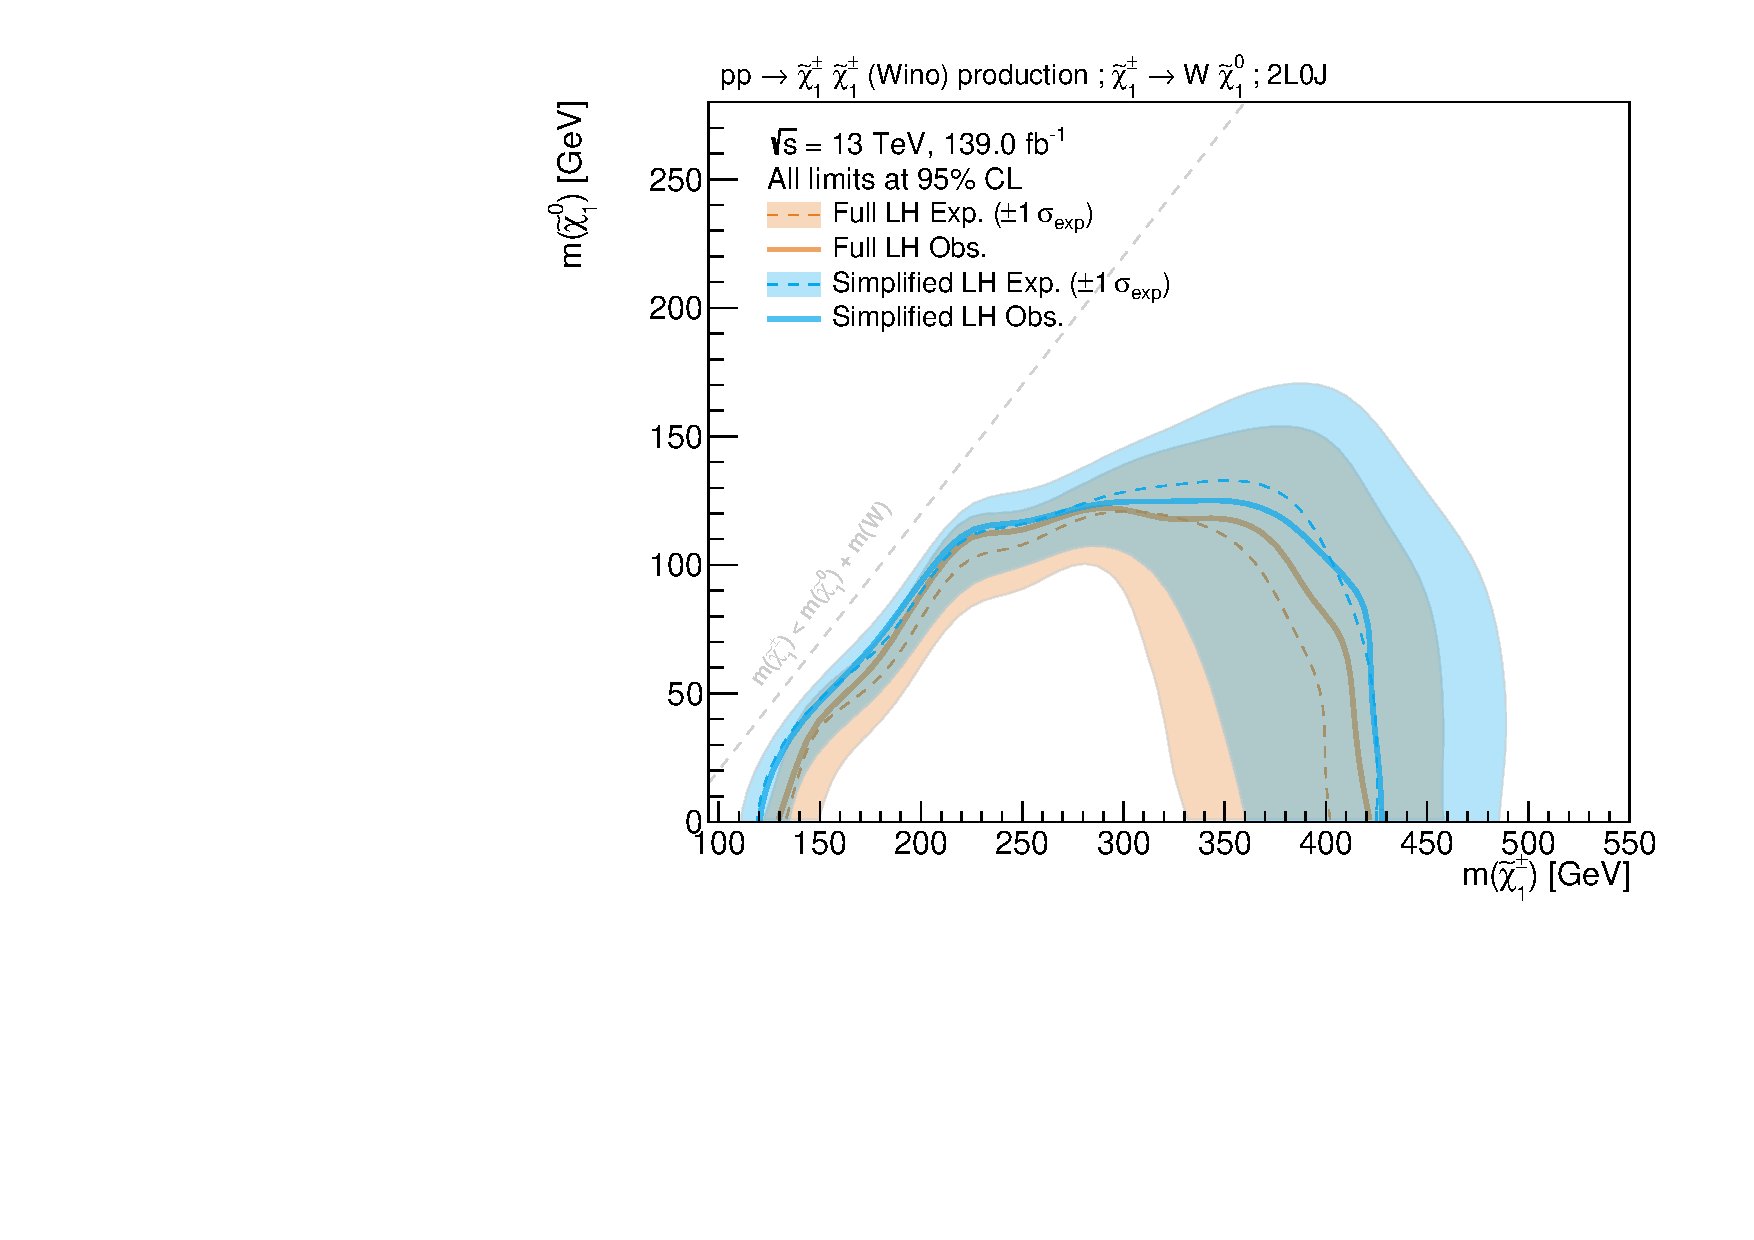
\includegraphics[width=\textwidth]{exclusion_2L0J_noLabel}
		\caption{ATLAS 2-lepton search~\cite{SUSY-2018-32}\label{fig:results_2L0J}}
	\end{subfigure}\hfill
	\begin{subfigure}[b]{0.5\textwidth}
		\centering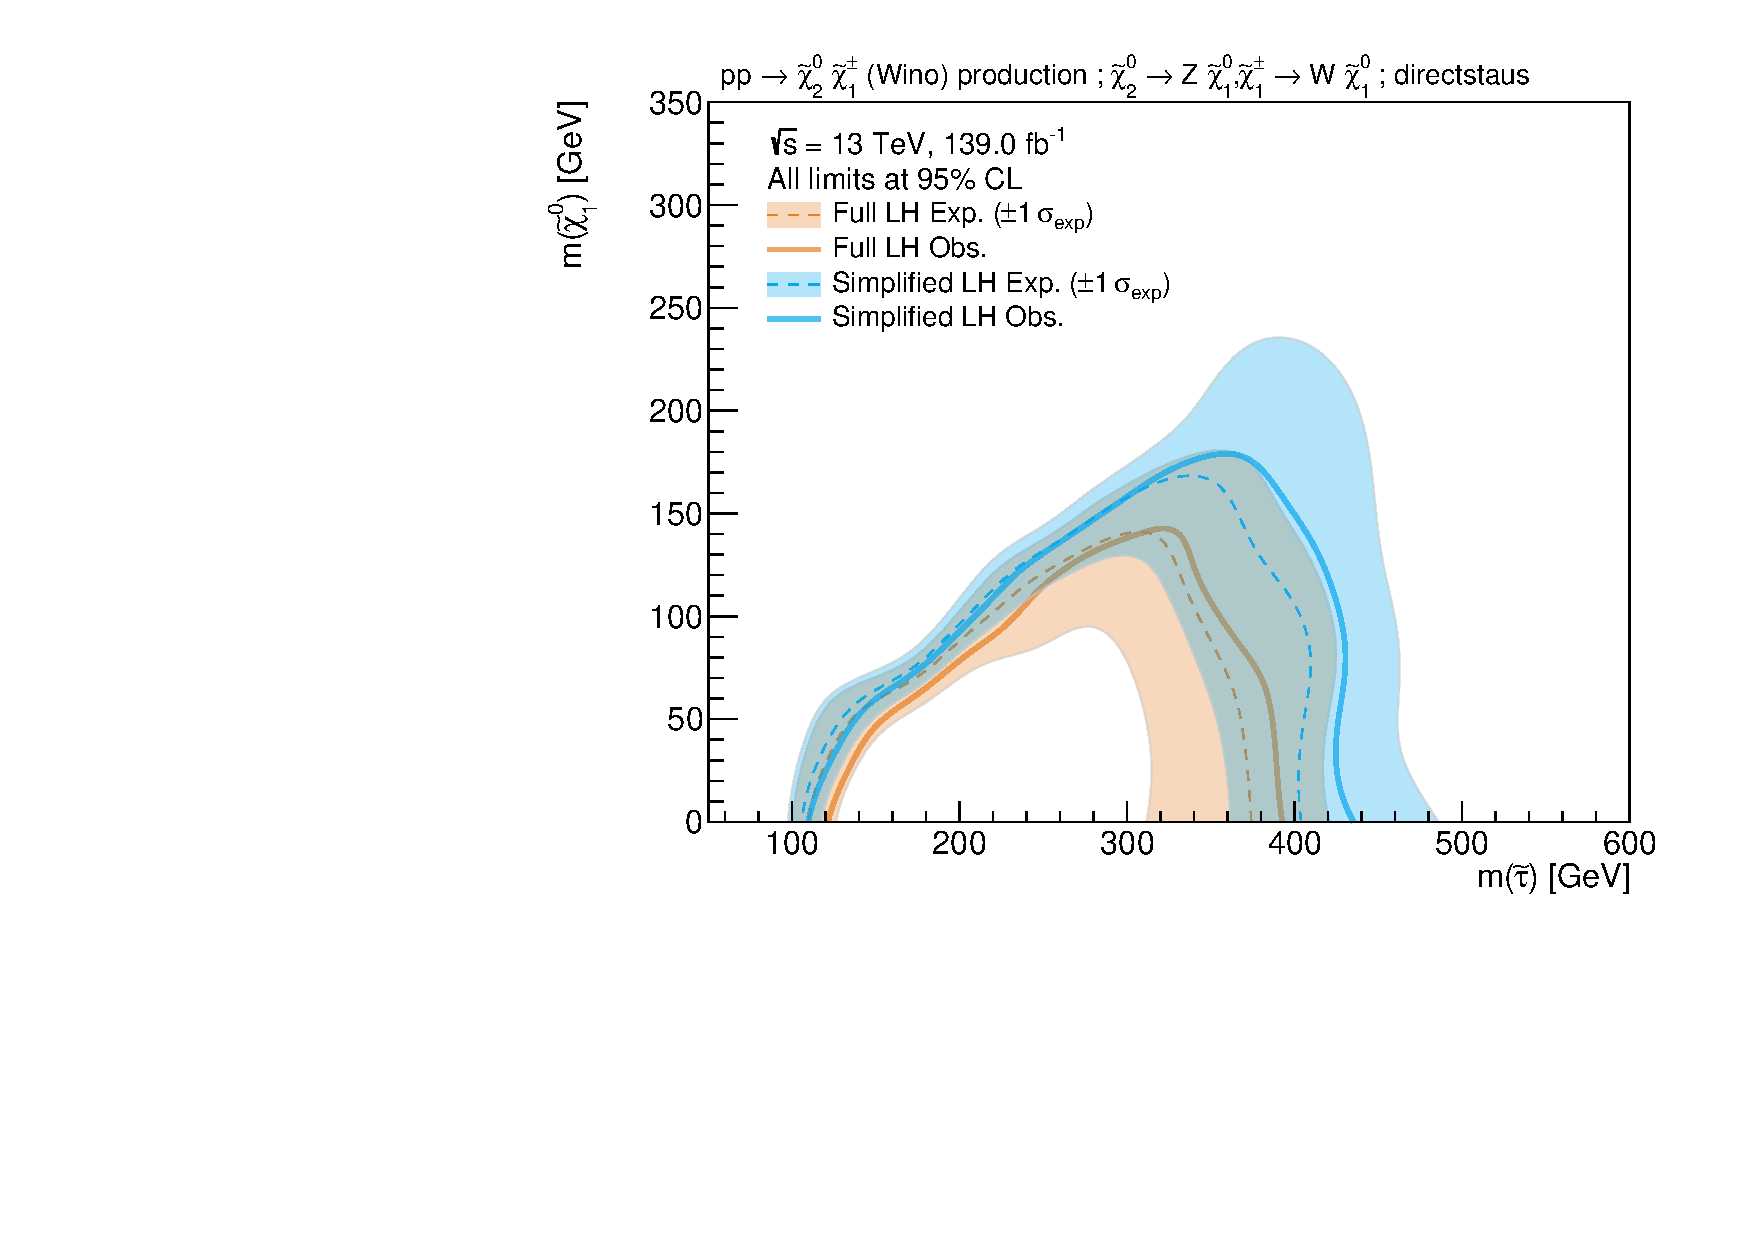
\includegraphics[width=\textwidth]{exclusion_directstaus_noLabel}
		\caption{ATLAS direct stau search~\cite{SUSY-2018-04}\label{fig:results_directstaus}}
	\end{subfigure}\hfill
	\begin{subfigure}[b]{0.5\textwidth}
		\centering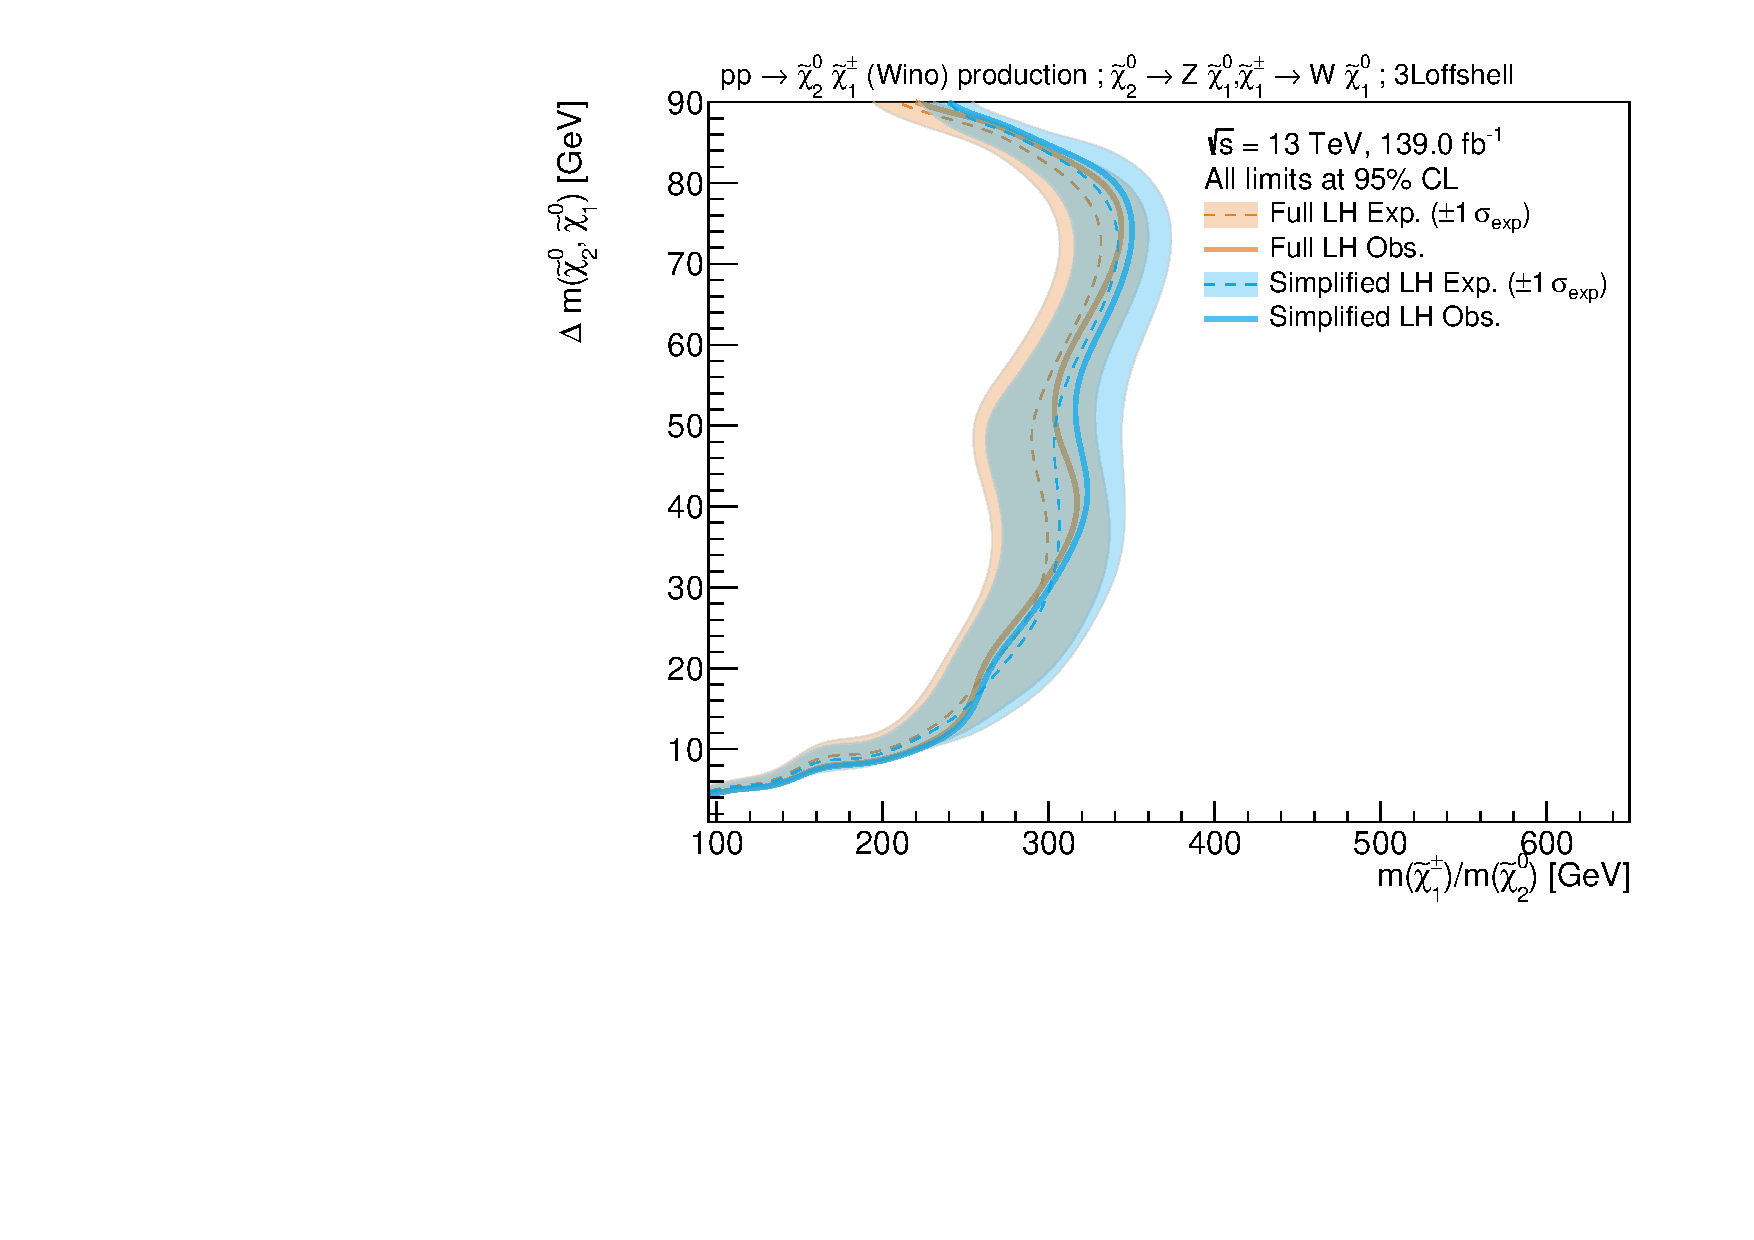
\includegraphics[width=\textwidth]{exclusion_3Loffshell_noLabel}
		\caption{ATLAS 3-lepton search\label{fig:results_3Loffshell}}
	\end{subfigure}\hfill
	\begin{subfigure}[b]{0.5\textwidth}
		\centering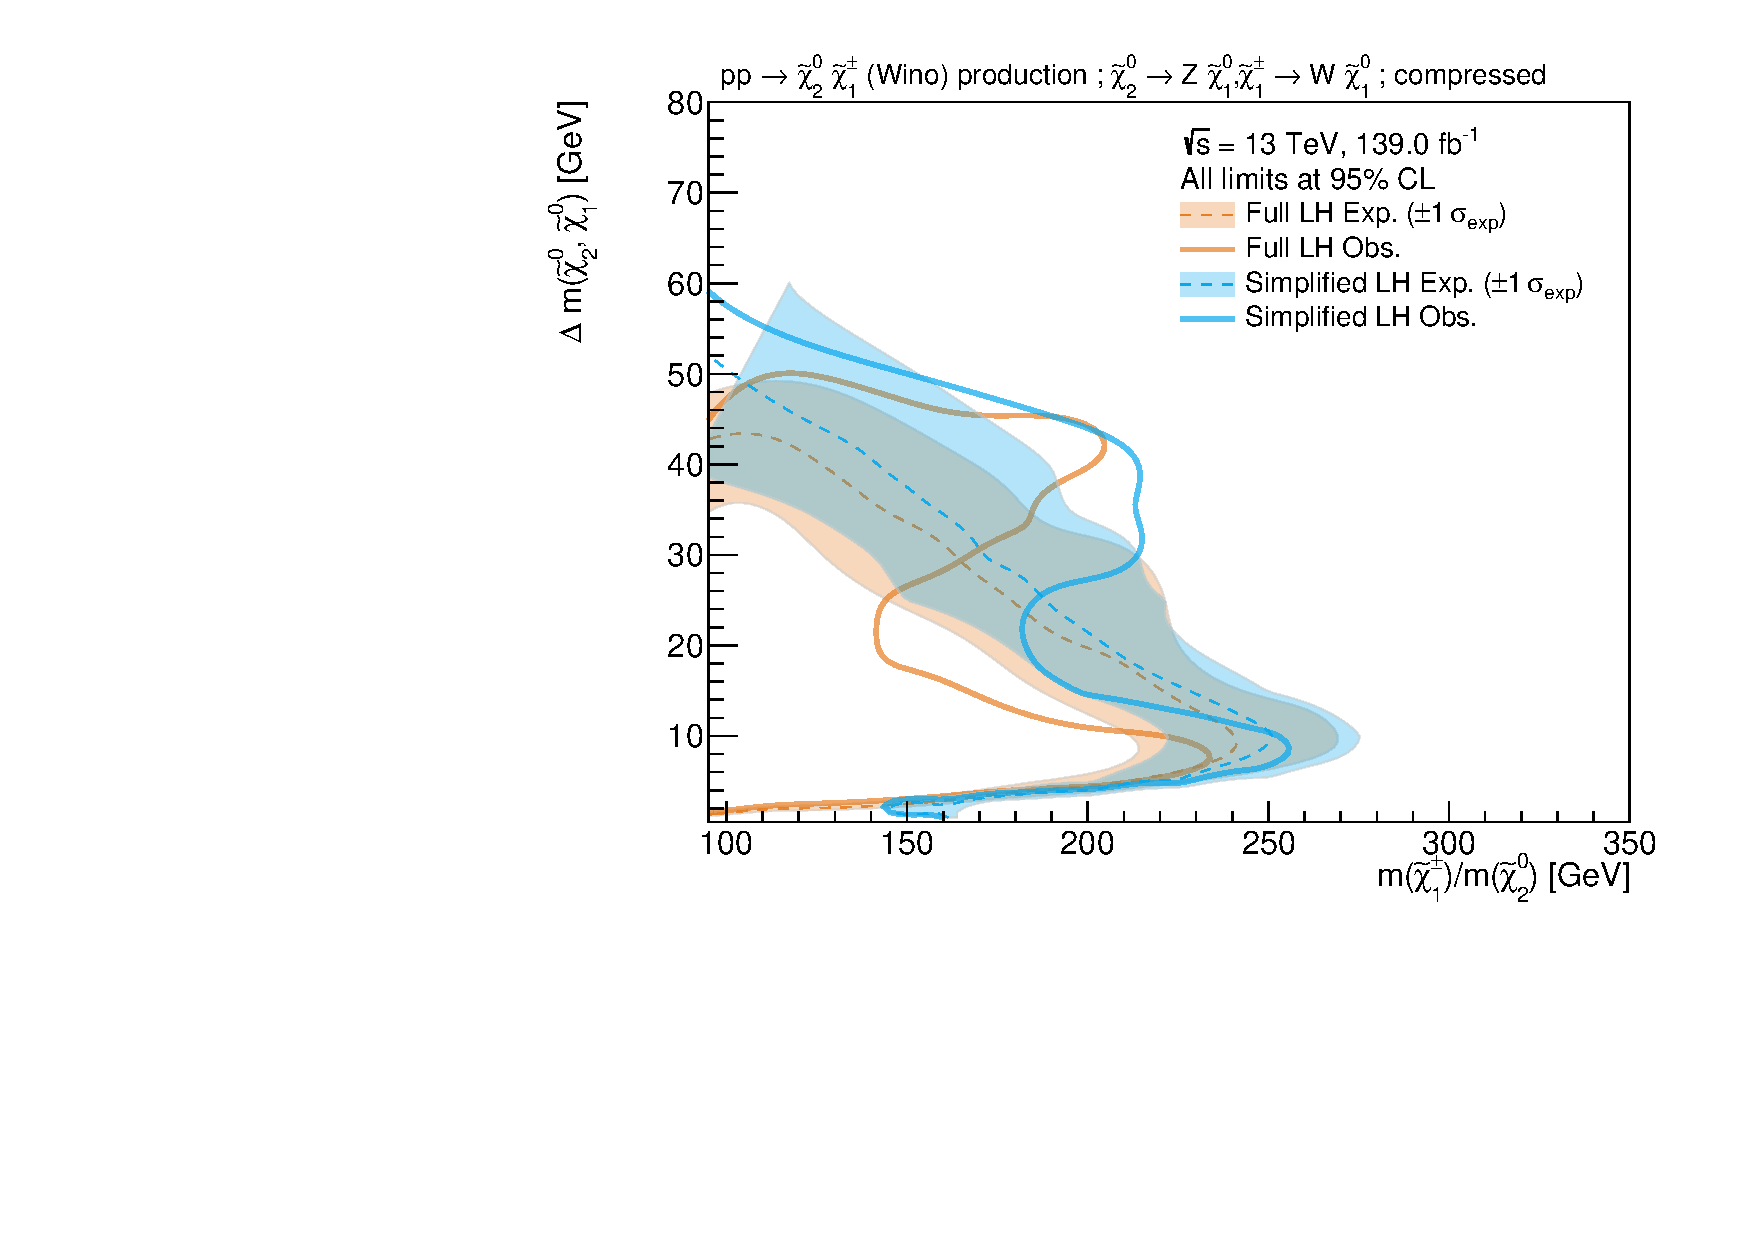
\includegraphics[width=\textwidth]{exclusion_compressed_noLabel}
		\caption{ATLAS compressed search~\cite{SUSY-2018-16}\label{fig:results_compressed}}
	\end{subfigure}\hfill
	\caption{Simplified likelihood results for the different ATLAS searches studied in this document. The results from the simplified likelihood (blue) are compared with the results of the full analysis likelihood (orange). The coloured numbers represent the observed CL$_s$ numbers obtained with both likelihoods.}\label{fig:results_analyses}
\end{figure}


\section{Limitations}\label{sec:simplify_limitations}

Building a well-performing simplified likelihood is not always as straightforward as described in~\cref{sec:building_simplified_likelihoods} and some analyses require special care when approximated. For example, in the case of the ATLAS compressed search~\cite{SUSY-2018-16} shown in~\cref{fig:results_compressed}, only a subset of the original analysis signal regions are entering the simplified likelihood, in order to improve the general agreement. The straightforward structure of the simplified likelihood is, in this case, not able to reproduce the statistical behaviour of the full likelihood. As the omitted channels only add limited sensitivity to the search, their removal in the simplified likelihood yields an overall improvement in agreement. 

The reason for this is that the simplified likelihood assumes that the background model can be described by a single sample with a single systematic uncertainty constrained by a Gaussian correlated over all bins, with background event rates and uncertainties obtained from a background-only fit in all \glspl{cr} and \glspl{sr} using the full likelihood. This in particular assumes that the background model is sufficiently constrained by the large statistics in the \glspl{cr} and that the introduction of signal contributions---especially in the \glspl{sr}---does not significantly change the background model in a way that cannot be replicated with a single background sample where the event rates only depend on a single nuisance parameter. While it can be argued that such an unstable fit configuration where \glspl{cr} are no longer sufficiently constraining the background should be avoided in an analysis, such a configuration is especially problematic for the simplified likelihood where the background model is assumed to be fixed up to a single constrained nuisance parameter.

\improvement{Plot of changing fit behaviour}

An additional limitation arises in cases of significant signal contamination in the \glspl{cr}. In the full likelihood, significant signal contamination in the \glspl{cr} generally leads to smaller best-fit background normalisation factors and thus smaller background estimates in the \glspl{sr}. This, in turn, results in conservative exclusion limits. In the simplified likelihood, even with the \glspl{cr} included, the single constrained nuisance parameter might in such cases not offer enough freedom to the fit to scale down the background model enough in the $\mu = 1$ fit, resulting in \textit{fake} sensitivity in the \glspl{cr}. Although it is generally important to limit signal contamination in the \glspl{cr} for the sake of healthy statistical fits, this is especially true in the case of very simplified likelihoods as introduced here. In the case of the ATLAS stop search shown in~\cref{fig:results_stop1L}, significant signal contamination of more than 30\% appears in many signal models with $m(\tilde{t}_1) < m(\lsp)+m(t)$\footnote{This is a kinematic region that the analysis is not designed to be sensitive in.}, which can thus not be evaluated with the simplified likelihood.

\section{Future prospects}

The simplified likelihoods introduced in this chapter can offer precise and extremely efficient approximations of ATLAS \gls{susy} searches for which the full likelihood in \texttt{JSON} format is available (either internally but preferably publicly). A proof-of-concept python tool has been developed for generic conversion of any full likelihood into the simplified format introduced here.

As the full likelihood defines the full statistical model given observed data in an analysis, other forms of likelihood simplifications can be thought of. One possible approach to investigate in the future is to construct likelihood simplifications with a variable number of nuisance parameters (as opposed to reducing the full set of nuisance parameters to a single one). In such an approach, a principal components analysis could be used to project the full $N$-dimensional nuisance parameter space onto a number $n$ principal components maximising the variance of the projected space, \ie resulting in minimal loss in correlation information. The $n$ principal components can then be kept separate, while the $N-n$ remaining components can be combined in quadrature into a \textit{residual} term. A similar approach was already introduced in \cref{ch:uncertainties} where the large number of nuisance parameters connected to the \gls{jer} and \gls{jes} uncertainties in the 1-lepton search were reduced to a more manageable set of \textit{effective} nuisance parameters with minimal loss in bin-by-bin correlation information. 

Up until very recently, the only way for physicists outside the collaboration to re-use ATLAS \gls{bsm} searches involved building approximations of their statistical models based on lossy projections of the full likelihood. With ATLAS' recent push to publish full analysis likelihoods, new approaches for approximation of the statistical models are becoming available. In principle, the full likelihood contains all information necessary for generating a simplified likelihood with an ideal compromise between statistical precision and computational efficiency, allowing to find an ideal approximation given constraints on available computing resources. 

\improvement{ref to simplify}




